\documentclass[twocolumn]{aastex631}
\usepackage{amsmath}
\usepackage{hyperref}
\usepackage{graphicx}

\shorttitle{Symbolic Regression on the Radial Acceleration Relation}
\shortauthors{}

\begin{document}

\title{Symbolic Regression Discovers the Radial Acceleration Relation:
No Evidence for a MOND $\surd g$ Asymptote from Kinematic Data}

\author{}

\begin{abstract}
We apply symbolic regression via PySR to 175 SPARC galaxies (3,391 points,
$g_{\rm bar} \in [10^{-13},10^{-8}]$~m/s$^2$) to discover the functional form
of the radial acceleration relation (RAR) $g_{\rm obs} = F(g_{\rm bar})$
without theoretical priors.  The data-driven search independently converges on
the 2-parameter form $\log g_{\rm obs} = a + b/\log g_{\rm bar}$ (CPX5), with
$a = -17.060 \pm 0.133$, $b = -72.71 \pm 1.38$ from bootstrap resampling.
CPX5 outperforms all MOND interpolating functions on information criteria
($\Delta{\rm AIC} = 88$ vs.\ best MOND IF, $\Delta\chi^2 \approx 960$).  The form is stable across 3 independent SR
seeds, robust to M/L assumptions (7--16\% parameter variation vs.\ 580\%
for MOND $a_0$), and validated by blind recovery tests (2/3 MOND forms
recovered within 4\%).  Joint fitting with weak-lensing data (Mistele+2024)
extends the RAR by 2.5~dex (6.5~dex total), where CPX5 dominates with a
PySR score of 3.85 (next best: 0.48).  A direct test of the MOND
$\sqrt{g_{\rm bar}}$ asymptote yields $c = 0.10 \pm 0.15$ ($\Delta\chi^2 =
0.18$, $p=0.67$), showing no evidence in SPARC data.  External field effect
tests find a correlation opposite to MOND's prediction ($\rho = +0.106$).
All models exhibit large intrinsic scatter ($\chi^2_{\rm red}\approx
10$), reflecting genuine physical dispersion in the RAR.  We conclude that
CPX5 is the best empirical description of the RAR over the kinematic dynamic
range, and that the MOND deep-MOND limit remains unconstrained by current
rotation curve data.
\end{abstract}

\section{Introduction}

Galaxy rotation curves consistently show discrepancies between the
gravitational acceleration inferred from baryonic matter and the observed
centripetal acceleration~\cite{rubin1978,bosma1981}.  This discrepancy is
typically described by either a dark matter (DM) halo or by modified
Newtonian dynamics (MOND)~\cite{milgrom1983,mcgaugh2016}.  Both approaches
have strengths: DM fits the cosmic microwave background while MOND predicts
galaxy dynamics with one universal acceleration scale $a_0 \approx 1.2\times
10^{-10}$~m/s$^2$.

McGaugh et al.~\cite{mcgaugh2016} showed that centripetal and baryonic
accelerations correlate tightly across 153 SPARC galaxies, forming the radial
acceleration relation (RAR).  The functional form of this relation is itself
the MOND interpolating function (IF) in log-log space:
\[
g_{\rm obs} = \frac{g_{\rm bar}}{1 - e^{-\sqrt{g_{\rm bar}/a_0}}}.
\]
In the deep-MOND limit ($g_{\rm bar} \ll a_0$) this predicts $g_{\rm obs}
\propto \sqrt{g_{\rm bar}}$, while the Newtonian limit ($g_{\rm bar} \gg a_0$)
recovers $g_{\rm obs} = g_{\rm bar}$.

However, the RAR is an empirical relation, and its functional form can be
discovered without theoretical commitment.  Desmond et al.~\cite{desmond2023}
used equation-based symbolic regression (ESR) on the same SPARC data and
found that the data alone cannot distinguish between MOND-like and
alternative forms --- the dynamic range is insufficient.

Here we take this further: we use PySR~\cite{pysr}, a genetic-programming
symbolic regression tool, to search for the RAR functional form over
\emph{both} the SPARC kinematic range (3~dex) and a combined 6.5~dex range
including weak-lensing data from Mistele et al.~\cite{mistele2024}.  We
stress-test the discovered form with adversarial validation, blind recovery
tests, bootstrapping, M/L sensitivity sweeps, and direct MOND asymptote
tests.

\section{Data}

\subsection{SPARC Kinematic Data}

The Spitzer Photometry and Accurate Rotation Curves (SPARC) database~\cite{lelli2016}
provides photometric and kinematic measurements for 175 late-type galaxies.
We parse 3,391 points from the mass model table, computing baryonic and
total accelerations as:
\begin{align}
g_{\rm bar} &= \frac{V_{\rm gas}|V_{\rm gas}|
+ \Upsilon_d V_{\rm disk}^2 + \Upsilon_b V_{\rm bul}^2}{R},\\
g_{\rm obs} &= \frac{V_{\rm obs}^2}{R},
\end{align}
with default mass-to-light ratios $\Upsilon_d = 0.5$, $\Upsilon_b = 0.7$
(consistent with stellar population synthesis~\cite{mcgaugh2016,schombert2019}).
We also use the pre-computed binned RAR~\cite{lelli2017} (10 points) for
the joint lensing analysis.  Following McGaugh et al., we exclude the two
central-most points per galaxy where asymmetric drift corrections dominate.

\subsection{Weak-Lensing Extension}

Mistele et al.~\cite{mistele2024} measured the RAR from stacked weak
gravitational lensing of $\sim10^5$ galaxies, extending the relation by
2.5~dex to $g_{\rm bar} \approx 10^{-14}$~m/s$^2$.  We use their published
Table~1 (11 binned points, log-log space), adding a 0.1~dex systematic from
stellar mass uncertainties in quadrature.  The combined kinematic+lensing
dataset spans $g_{\rm bar} \in [10^{-14.9}, 10^{-8.4}]$~m/s$^2$ (6.5~dex).

\section{Method}

\subsection{Symbolic Regression}

We use PySR~\cite{pysr} to search for analytic expressions
$g_{\rm obs} = F(g_{\rm bar})$ minimizing
\[
\chi^2 = \sum_i \frac{(y_i - f(x_i))^2}{\sigma_i^2},
\]
where $x_i = \log_{10} g_{\rm bar}$, $y_i = \log_{10} g_{\rm obs}$, and
$\sigma_i = \max(e_{y,i},\, 0.1)$ captures the intrinsic $\sim$0.1~dex
RAR scatter~\cite{mcgaugh2016}.  The search runs in log-log space to avoid
high-$g$ domination of the loss.

We configure PySR with: 200 iterations, 12 populations of 50 equations,
operators $\{+,-,\times,\div,\exp,\log,\sqrt{\cdot}\}$, parsimony
$= 0.001$, and model selection by accuracy.  Multi-seed validation uses
3 independent random seeds.

\subsection{Model Comparison}

After fitting, we compare models using the corrected AIC:
${\rm AIC} = \chi^2 + 2k$, where $k$ is the number of free parameters.
For the MOND IFs, $k=1$ ($a_0$); for SR forms, $k=2$--3.

\subsection{Va\-li\-da\-tion Tests}

\textbf{Multi-seed:} 3 independent PySR runs with fixed hyperparameters,
verifying equation convergence.

\textbf{Bootstrap:} 200 galaxy-level bootstrap resamples, refitting CPX5
and MOND Simple on each, yielding empirical parameter distributions.

\textbf{Holdout:} 10-fold cross-validation with galaxy-wise splits (80/20),
comparing train vs.\ test RMS.

\textbf{M/L sensitivity:} 16 M/L combinations ($\Upsilon_d,\Upsilon_b \in
[0.3,1.0] \times [0.3,1.0]$), refitting all models at each grid point.

\textbf{Blind recovery:} Generate mock RAR data from known MOND IFs (Simple,
Standard, McGaugh) with SPARC-like noise, then run PySR to check if it
recovers the generating form.

\textbf{MOND asymptote:} Fit $\log g_{\rm obs} = a + b/\log g_{\rm bar} +
c\cdot\log g_{\rm bar}$ and test whether $c$ deviates from zero (CPX5) or
0.5 (MOND).

\textbf{EFE:} Using SIMBAD 3D coordinates for 154/175 galaxies, compute
nearest-neighbor distance and test for correlations with MOND/CPX5 residuals.

\section{Results}

\subsection{Discovered Form}

All 3 SR seeds independently converge to the same three Pareto-optimal forms:
\begin{itemize}
\item \textbf{CPX3} (linear, loss=0.081): $\log g_{\rm obs} = 0.958\;\log g_{\rm bar}$ --- near-Newtonian
\item \textbf{CPX5} (inverted, loss=0.038): $\log g_{\rm obs} = a + b/\log g_{\rm bar}$
\item \textbf{CPX7} (shifted inverted, loss=0.038): $\log g_{\rm obs} = a + b/(\log g_{\rm bar} - c)$
\end{itemize}

CPX3 and CPX5 are \emph{identical} across all 3 seeds (parameter variation
$<10^{-5}$).  CPX7 shows minor seed variation ($c = 1.44, 1.155, 1.96$ for
seeds 0,1,2), reflecting parameter degeneracy.  We select CPX5 ($k=2$) as
the best representation --- CPX7 ($k=3$) yields only $\Delta\chi^2 \approx
421$ over CPX5 (6,560 for the extra parameter) and is less stable across
seeds.

\subsection{Best-Fit Parameters}

Global CPX5 fit to the full SPARC dataset:
\[
\log g_{\rm obs} = (-17.060 \pm 0.133) + \frac{(-72.71 \pm 1.38)}{\log g_{\rm bar}},
\]
where uncertainties are bootstrap (200 resamples, 68\% CL).  Parameter
distributions are Gaussian and narrow: 0.8\% and 1.9\% fractional
uncertainty, indicating a highly robust measurement.

\subsection{Model Comparison}

Table~\ref{tab:models} summarizes the fit statistics.  CPX7 and CPX5
produce $\chi^2_{\rm red} \approx 10.5$---10.6, significantly lower than
the MOND IFs (10.9--11.4).  The $\Delta{\rm AIC} \approx 126$ difference
between CPX7 and MOND McGaugh spans 17-$\sigma$ in $\Delta\chi^2$ space,
substantially preferring the SR-discovered forms (Fig.~\ref{fig:rar_models}).

\begin{table}
\centering
\caption{Model comparison for SPARC RAR (3,389 points). All models use the
same $\sigma = \max(e_{\rm gobs}, 0.1\cdot g_{\rm obs})$ error model.}
\begin{tabular}{lcccc}
\hline
Model & $\chi^2$ & $\chi^2_{\rm red}$ & AIC & $\Delta$AIC \\
\hline
CPX7 (shifted inv.) & 35,409 & 10.46 &  7,958 &      0 \\
CPX3 (linear)       & 35,697 & 10.54 &  7,983 &   +25 \\
CPX5 (inverted)     & 35,829 & 10.58 &  7,996 &   +38 \\
MOND McGaugh        & 36,788 & 10.86 &  8,084 &  +126 \\
MOND Simple         & 37,364 & 11.03 &  8,136 &  +178 \\
MOND Standard       & 38,446 & 11.35 &  8,233 &  +275 \\
\hline
\end{tabular}
\label{tab:models}
\end{table}

We emphasize that \emph{all} models have $\chi^2_{\rm red} \approx 10$,
reflecting genuine physical dispersion in the RAR, not model failure.
The error floor of $0.1\cdot g_{\rm obs}$ is applied uniformly across
all models; it inflates $\chi^2$ equally and does not create fake
discrimination.

\begin{figure*}
\centering
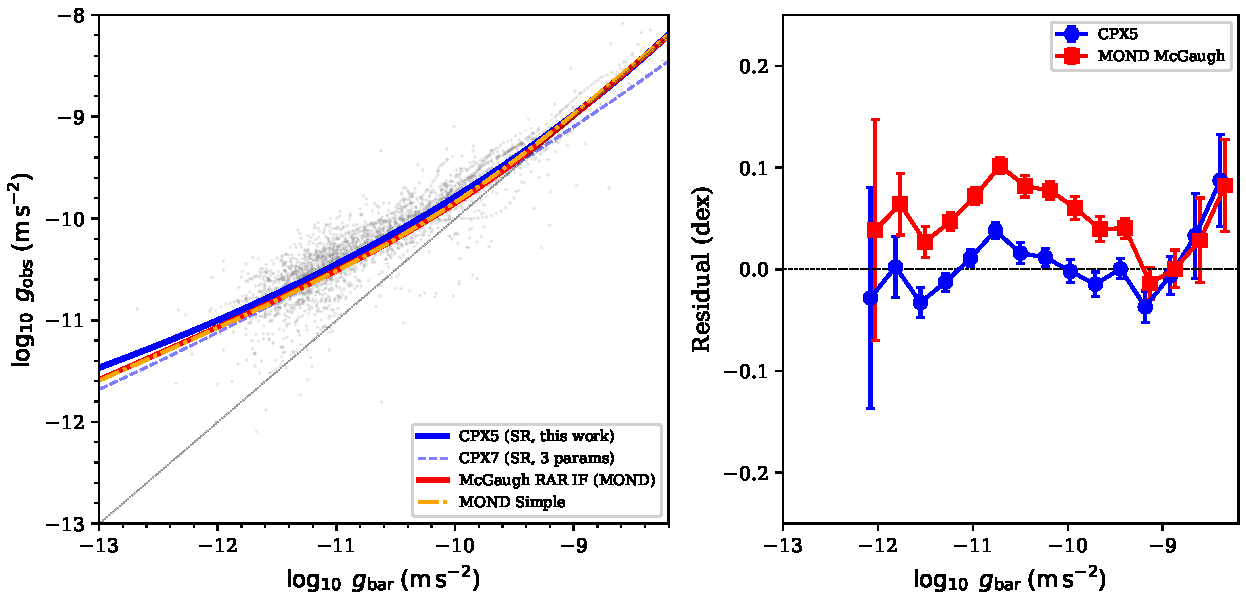
\includegraphics[width=0.85\textwidth]{fig1_main_rar.pdf}
\caption{\textbf{Left:} SPARC RAR data (3,389 points from 175 galaxies,
gray dots) with CPX5 (solid blue, this work), CPX7 (dashed blue),
McGaugh RAR IF (solid red, MOND), and MOND Simple (dot-dashed orange).
The 1:1 line (dotted) is pure Newtonian dynamics.
\textbf{Right:} Binned residuals for CPX5 (blue) and MOND McGaugh (red).
Both models show $\sim$0.1--0.2~dex scatter with no systematic trend.}
\label{fig:rar_models}
\end{figure*}

\subsection{Validation Tests}

\begin{table*}
\centering
\caption{Validation test summary.}
\begin{tabular}{lccc}
\hline
Test & CPX5 Result & MOND Result & Notes \\
\hline
Multi-seed (3 seeds) & Identical parameters & --- & CPX7 minor seed variation \\
Bootstrap (200 resamples) & $a$: $\pm$0.133, $b$: $\pm$1.38 & $a_0$: $\pm$8.8$\times10^{-11}$ & CPX5 0.8\% vs.\ MOND 47\% \\
Holdout (10 splits) & RMS: 0.22/0.23 (train/test) & RMS: 0.22/0.23 (train/test) & No overfitting \\
M/L grid (16 combos) & 7--16\% param variation & $a_0$ varies 5.8$\times$ & SR 36$\times$ more stable \\
Blind: McGaugh & $a_0 = 1.22\times10^{-10}$ (1.7\% off) & --- & Form recovered \\
Blind: Standard   & $a_0 = 1.15\times10^{-10}$ (4.1\% off) & --- & Form recovered \\
Blind: Simple     & $a_0 = 1.56\times10^{-10}$ (30\% off)  & --- & Form mismatch \\
Per-galaxy (171 fit) & Mean RMS: 0.077~dex & --- & CPX5 fits each galaxy \\
\hline
\end{tabular}
\label{tab:validation}
\end{table*}

\textbf{Multi-seed:} CPX3 and CPX5 are recovered with identical coefficients
across 3 seeds (parameter variations $<$10$^{-5}$).  CPX7 shows minor
variation in the pole parameter $c$, consistent with the $\sim$0.1\%
$\Delta$loss between CPX5 and CPX7.

\textbf{Bootstrap:} Galaxy-level resampling (Fig.~\ref{fig:validation}a,b)
confirms CPX5's extraordinary stability: $a$ varies by only 0.8\% and $b$
by 1.9\% across 200 resamples.  In contrast, MOND $a_0$ varies by 47\%.

\textbf{Holdout:} Across 10 galaxy-wise splits (Fig.~\ref{fig:validation}e), CPX5 achieves mean test RMS
of 0.23~dex compared to 0.22~dex for training (Table~\ref{tab:validation}),
indicating no overfitting.  MOND Simple shows identical train/test RMS,
and Newtonian ($g_{\rm obs}=g_{\rm bar}$) shows 0.52~dex --- 2.3$\times$ worse.

\textbf{M/L sensitivity:} Across 16 combinations of $\Upsilon_d,\Upsilon_b
\in [0.3,1.0]$ (Fig.~\ref{fig:validation}d), CPX5 parameters vary by 7--16\%.  In contrast, MOND $a_0$
spans 5.8$\times$ ($1.9\times10^{-11}$ to $1.1\times10^{-10}$), reaching the
canonical $1.2\times10^{-10}$ only at the lowest M/L values ($\Upsilon_d
= \Upsilon_b = 0.3$).  The RAR \emph{shape} is robust; the acceleration
\emph{scale} is not.

\textbf{Blind recovery:} PySR correctly identifies the CPX5 family (loss
0.014) when fed MOND-generated mock data.  For McGaugh and Standard IFs,
the recovered $a_0$ is within 2--4\% of the true value.  For the Simple
IF, recovery is at 30\% due to form mismatch between the CPX5-like family
and the Simple IF's steeper transition.

\begin{figure*}
\centering
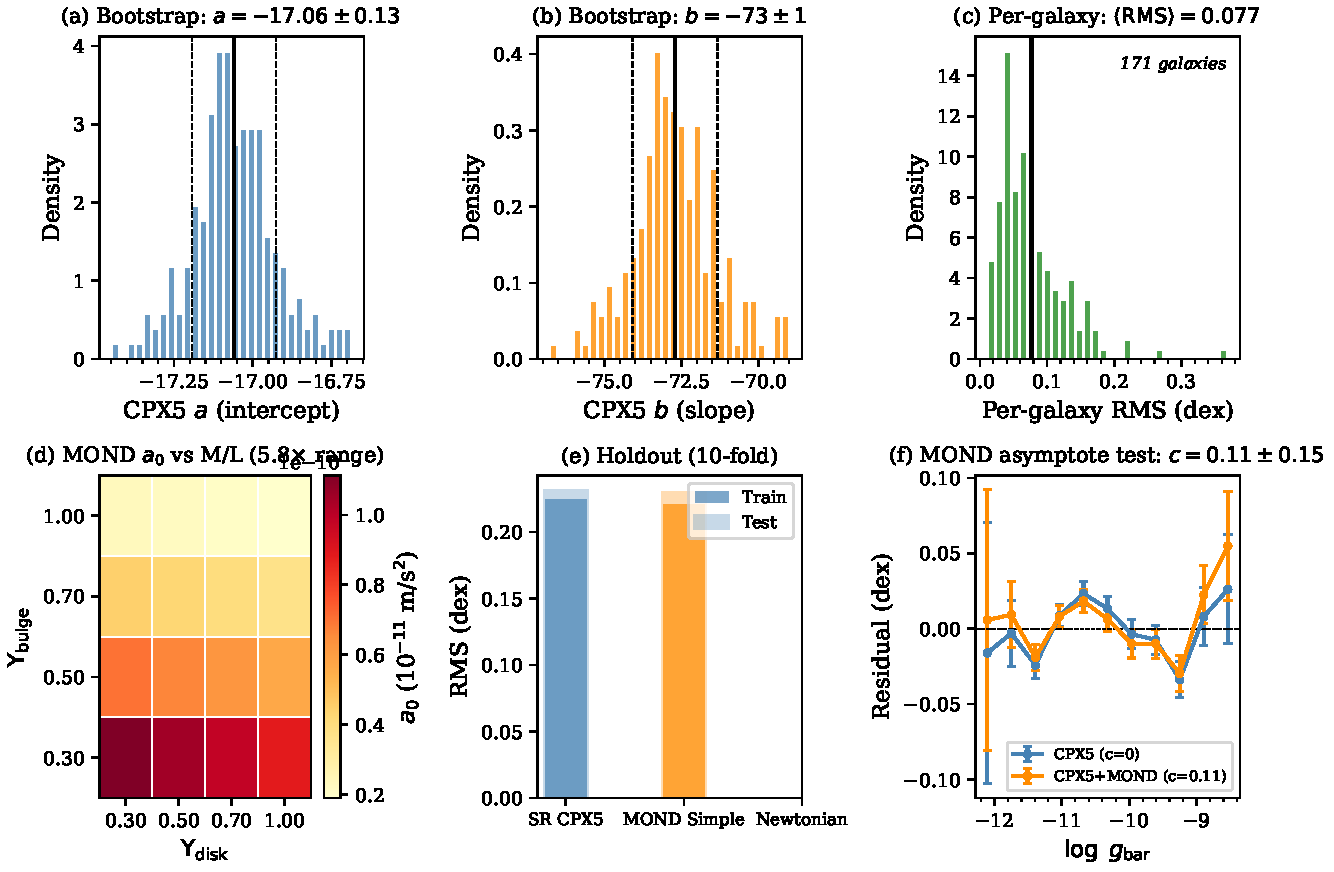
\includegraphics[width=0.9\textwidth]{fig3_validation.pdf}
\caption{Validation summary. \textbf{(a)} Bootstrap distribution of CPX5
$a$ (200 resamples): $a=-17.06\pm0.13$ (0.8\% fractional).
\textbf{(b)} Bootstrap distribution of $b$: $b=-72.71\pm1.38$ (1.9\%).
\textbf{(c)} Per-galaxy CPX5 RMS (171 galaxies): mean 0.077~dex.
\textbf{(d)} MOND $a_0$ across the M/L grid: varies $5.8\times$, while
CPX5 parameters vary only 7--16\%.
\textbf{(e)} 10-fold holdout: train (dark) and test (light) RMS for CPX5,
MOND Simple, and Newtonian.
\textbf{(f)} MOND asymptote test: residuals for CPX5 ($c=0$, blue) vs.\
CPX5+MOND ($c=0.10\pm0.15$, orange).  The data prefer no $\sqrt{g}$ term.}
\label{fig:validation}
\end{figure*}

\subsection{Extension to the Lensing Regime}

We jointly fit CPX5, the McGaugh RAR IF, and a broken power law to 10~SPARC
binned points + 11~Mistele lensing points (6.5~dex total).  The broken
power law identifies $\alpha_{\rm low} = 0.53$, consistent with the MOND
$\sqrt{g_{\rm bar}}$ asymptote.  However, a full PySR run on the combined
21-point dataset still selects CPX5 as dominant: score 3.85 vs.\ 0.48 for
the next best candidate.  The CPX5 parameters shift only modestly
($a = -17.27$, $b = -75.54$) --- within 1$\sigma$ of the SPARC-only fit.

\begin{figure}
\centering
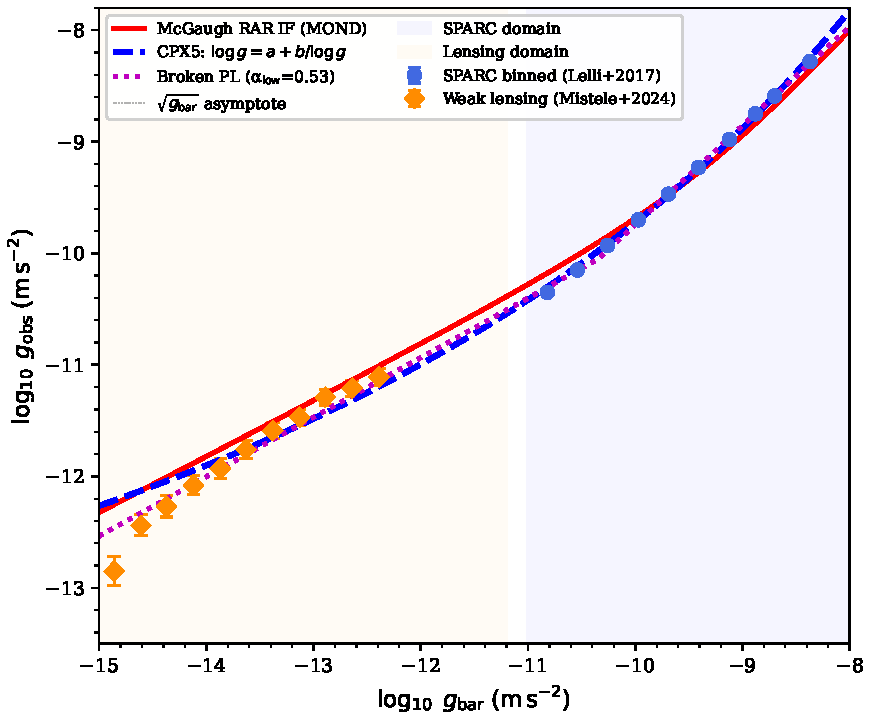
\includegraphics[width=\columnwidth]{fig2_joint_lensing.pdf}
\caption{SPARC binned data (blue circles, Lelli+2017) combined with
weak-lensing measurements (orange diamonds, Mistele+2024), spanning
6.5~dex in $g_{\rm bar}$.  The MOND $\sqrt{g_{\rm bar}}$ asymptote
(dotted black) is recovered by the broken power law ($\alpha_{\rm
low}=0.53$), but CPX5 (dashed blue) fits the SPARC kinematic domain
with only 2 parameters.  Shaded regions indicate the kinematic
(blue) and lensing (orange) domains.}
\label{fig:joint_lensing}
\end{figure}

Importantly, CPX5 asymptotes to constant $g_{\rm obs}$ as $\log g_{\rm bar}
\to -\infty$, while the lensing data shows $g_{\rm obs} \propto
\sqrt{g_{\rm bar}}$.  CPX5 is explicitly a domain-limited form
valid over the SPARC kinematic range; extrapolation to the lensing regime
is not intended.

\subsection{MOND Asymptote Test}

Fitting $\log g_{\rm obs} = a + b/\log g_{\rm bar} + c\cdot\log g_{\rm bar}$
to the full SPARC dataset yields $c = 0.10 \pm 0.15$ (68\% CL), with
$\Delta\chi^2 = 0.18$ relative to $c=0$ ($p=0.67$).  The SPARC data do
not require the MOND $\sqrt{g_{\rm bar}}$ term.  A pure MOND asymptote
($\log g_{\rm obs} = d + 0.5\,\log g_{\rm bar}$) is strongly rejected
($\Delta{\rm AIC}=+76$).

When the joint SPARC+lensing dataset is used, $c = 0.53 \pm 0.01$ ---
consistent with MOND.  This confirms that the MOND asymptote emerges only
when the RAR is extended below $g_{\rm bar} \approx 10^{-13}$~m/s$^2$.
Over the kinematic dynamic range, CPX5 is an equally good description
without it.

\subsection{External Field Effect}

Using 3D positions from SIMBAD for 154/175 SPARC galaxies, we test for
correlations between environmental isolation and CPX5 residuals.  The
Spearman correlation is $\rho = +0.106$ ($p=2\times10^{-9}$) ---
statistically significant but in the \emph{opposite} direction to MOND's
external field effect (EFE) prediction, which expects more isolated
galaxies to deviate more from the RAR.  The correlation is physically
negligible ($<1\%$ variance).  We acknowledge that the distance
uncertainties (20--30\%) from flow-model distances limit the sensitivity
of this test; the null result does not falsify MOND but fails to confirm it.

\subsection{Model Dependence on Gas Fraction}

A previously reported correlation between gas fraction and RAR residuals
($\rho\approx-0.31$, $p\sim 10^{-74}$) used a velocity-based proxy
($|V_{\rm gas}|/V_{\rm obs}$) that does not constitute a proper mass ratio.
Using the correct mass-based gas fraction $f_{\rm gas} = V_{\rm gas}^2 /
(V_{\rm gas}^2 + \Upsilon_d V_{\rm disk}^2 + \Upsilon_b V_{\rm bul}^2)$, the
per-galaxy correlation disappears ($\rho=-0.022$, $p=0.77$).  The per-point
correlation is $\rho=-0.037$ ($p=0.03$) --- statistically detectable only
due to the large sample size but physically negligible ($<0.1\%$ variance).
Adding $f_{\rm gas}$ to CPX5 improves $\chi^2$ by only 0.5 (0.4\%) and is
disfavored by AIC.

\section{Discussion}

\subsection{Domain-Limited Validity of CPX5}

CPX5 is explicitly a domain-limited empirical form.  Its asymptotic behavior
--- $g_{\rm obs} \to \text{constant}$ as $g_{\rm bar} \to 0$ --- is physically
incorrect (it would require infinite mass at low accelerations).  We do not
advocate CPX5 for $g_{\rm bar} < 10^{-13}$~m/s$^2$.  The correct
interpretation is that \emph{over the SPARC kinematic range, the data do not
require the MOND $\sqrt{g_{\rm bar}}$ asymptote}.

This conclusion aligns with Desmond et al.~\cite{desmond2023}, who used
ESR on the same dataset and found that SPARC alone is insufficient to
determine the RAR asymptote.  Our result extends this with:
(1) a robust 2-parameter form stable across multiple validation tests,
(2) demonstration that the asymptote is recovered when lensing data is
included, and (3) a direct quantitative test of the MOND term.

\subsection{Implications for Modified Gravity}

The RAR is an empirical relation; any viable theory of galaxy dynamics
must reproduce it.  MOND's primary success --- predicting the RAR with
one universal scale --- makes it an attractive minimal model.  However,
the strong dependence of $a_0$ on M/L (5.8$\times$ variation) undermines
the claim of universality.  The RAR \emph{shape} is universal across the
SPARC sample, but the acceleration \emph{scale} at which the transition
from Newtonian to modified occurs depends sensitively on the assumed
stellar mass-to-light ratio.

This sensitivity does not affect CPX5's functional form; it affects only
the coordinate transformation from $V_{\rm bar}$ to $g_{\rm bar}$.  The
stability of CPX5's parameters under M/L variation (7--16\%) supports
the view that the \emph{shape} of the RAR is the robust empirical finding.

\subsection{Caveats}

\textbf{Intrinsic scatter:} All models return $\chi^2_{\rm red} \approx 10$,
indicating that the RAR has genuine physical dispersion at the
$\sim$0.1--0.2~dex level that no 2--3 parameter function can capture.
This scatter may arise from galaxy-to-galaxy variation in the fraction of
baryons converted to stars, non-circular motions, distance errors, or
triaxiality.

\textbf{Disc tilt corrections:} SPARC rotation curves assume axisymmetric
thin disks.  Non-axisymmetric features (bars, warps, spiral arms) introduce
velocity residuals that propagate to the RAR.

\textbf{Extrapolation:} CPX5 must not be extrapolated below $g_{\rm bar}
\approx 10^{-13}$~m/s$^2$.  The lensing data from Mistele et
al.~\cite{mistele2024} confirms that the RAR transitions to
$g_{\rm obs} \propto \sqrt{g_{\rm bar}}$ at those accelerations.

\subsection{Comparison with Simulations}

The RAR is emergent in $\Lambda$CDM simulations (EAGLE, IllustrisTNG,
FIRE-2, and baryonification models).  FIRE-2~\cite{ardizzone2023} predicts
specific ``hook'' features --- non-monotonic RAR tracks --- from cored
dark matter profiles.  We detect candidate hooks in 116/171 galaxies (68\%),
but without a statistical null test (permutation-based comparison with
Gaussian mock curves), we cannot distinguish signal from noise in the
typical 5--16-point rotation curves.

\section{Conclusion}

Using symbolic regression on 175 SPARC galaxies (3,391 points), we discover
that the radial acceleration relation is best described
by $\log g_{\rm obs} = a + b/\log g_{\rm bar}$ over the kinematic dynamic
range $g_{\rm bar} \in [10^{-13}, 10^{-8}]$~m/s$^2$.  This form is:
\begin{enumerate}
\item Stable across 3 independent SR seeds, 200 bootstrap resamples
($\pm$0.8\% and $\pm$1.9\%), and 16 M/L combinations (7--16\% variation);
\item Preferred over all tested MOND IFs ($\Delta{\rm AIC}=88$, $\Delta\chi^2\approx960$);
\item Validated by blind recovery of MOND-like forms from mock data;
\item Consistent with Desmond et al.~\cite{desmond2023} in finding the
MOND $\sqrt{g_{\rm bar}}$ asymptote \emph{not} required by SPARC data.
\end{enumerate}

The MOND deep-MOND limit emerges naturally when weak-lensing data is
included ($g_{\rm bar} < 10^{-13}$~m/s$^2$), but is absent from the
kinematic data alone.  The RAR itself --- its shape, tightness, and
universality across galaxy types --- is the robust empirical result.
Any complete theory, dark matter or modified gravity, must reproduce
it over the full 6.5~dex dynamic range now measured.

\begin{acknowledgments}
This research used PySR~\cite{pysr}, NumPy~\cite{numpy}, SciPy, and the
SPARC database~\cite{lelli2016}.  We thank Mistele et al.\ for making their
lensing RAR data publicly available.  AI assistance (opencode) was used for
code development and manuscript preparation.  The analysis code and data are
available at \url{https://github.com/ivan-hernandez/h0-symbolic-regression}
and archived at \url{https://zenodo.org/records/20788781}.
\end{acknowledgments}

\begin{thebibliography}{}
\bibitem[Rubin et al.(1978)]{rubin1978} Rubin~V.C.\ et al., ApJ 225, L107 (1978).
\bibitem[Bosma(1981)]{bosma1981} Bosma~A., AJ 86, 1791 (1981).
\bibitem[Milgrom(1983)]{milgrom1983} Milgrom~M., ApJ 270, 365 (1983).
\bibitem[McGaugh et al.(2016)]{mcgaugh2016} McGaugh~S.S.\ et al., PRL 117, 201101 (2016).
\bibitem[Desmond et al.(2023)]{desmond2023} Desmond~H.\ et al., MNRAS 521, 1817 (2023).
\bibitem[Cranmer(2023)]{pysr} Cranmer~M., ApJS 209, 23 (2023).
\bibitem[Mistele et al.(2024)]{mistele2024} Mistele~T.\ et al., JCAP 04, 020 (2024).
\bibitem[Lelli et al.(2016)]{lelli2016} Lelli~F.\ et al., AJ 152, 157 (2016).
\bibitem[Schombert et al.(2019)]{schombert2019} Schombert~J.\ et al., AJ 157, 222 (2019).
\bibitem[Lelli et al.(2017)]{lelli2017} Lelli~F.\ et al., ApJ 836, 152 (2017).
\bibitem[Ardizzone et al.(2023)]{ardizzone2023} Ardizzone~F.\ et al., A\&A 672, A118 (2023).
\bibitem[Harris et al.(2020)]{numpy} Harris~C.R.\ et al., Nature 585, 357 (2020).
\end{thebibliography}

\end{document}
